% gepisat-3_stage2.tex
%
% written by Tyler W. Davis
% Imperial College London
%
% 2014-10-29 -- created
% 2015-03-18 -- last updated
%
% ------------
% description:
% ------------
% This TEX file contains Part 3 modeling Stage 2 for the GePiSaT model documentation.
%
% ----------
% changelog:
% ----------
% 01. modularized chapter [14.10.29]
% 02. newline for each sentence [14.10.29]
% --> simpler for Git version control
% 03. changed LUE figure from CH-Oe1 to CA-Qfo [14.10.29]
% 04. moved fPAR to data section in Part 1 [15.03.18]
%
%% \\\\\\\\\\\\\\\\\\\\\\\\\\\\\\\\\\\\\\\\\\\\\\\\\\\\\\\\\\\\\\\\\\\\\\\\ %%
%% PART 3.3 -- STAGE 2
%% //////////////////////////////////////////////////////////////////////// %%
\section{Stage 2: Light-Use Efficiency}
\label{sec:mst2}
In stage 2, a production efficiency model (PEM) or ``diagnostic'' model of monthly light-use efficiency (LUE) estimates is developed.  
The basic LUE model is based on gap-filled and time-aggregated GPP, PPFD, and fPAR.  
The basic PEM algorithm is defined as \parencite[Eq. 1]{mccallum09}:
%% ------------------------------------------------------------------------ %%
%% eq:pem | Production efficiency model
%% ------------------------------------------------------------------------ %%
\nomenclature{$\varepsilon$}{LUE [mol CO$_{2}\cdot$m$^{-2}\cdot$mol PPFD$^{-1}$]}
\begin{equation}
\label{eq:pem}
    \text{GPP} = \varepsilon \cdot \text{fPAR} \cdot \text{PPFD} 
\end{equation}

\noindent where:\\
\indent GPP = gross primary production [mol CO$_{2}\cdot$m$^{-2}$]\\
\indent $\varepsilon$ = LUE [mol CO$_{2}\cdot$m$^{-2}\cdot$mol PPFD$^{-1}$]\\
\indent fPAR = fractionally absorbed PAR\\
\indent PPFD = photosynthetic photon flux density [mol$\cdot$m$^{-2}$]\\

\noindent In this model, GPP, fPAR, and PPFD represent monthly values.  
Figure \ref{fig:lue} shows an example of the basic LUE regression defined in equation \ref{eq:pem}.  
The 22 months of data are taken from a flux tower located in Quebec, Canada (CA-Qfo).  
The correlation between monthly integrated GPP and monthly integrated fPAR $\times$ PPFD is strongly linear ($r = 0.97$).
%% ------------------------------------------------------------------------ %%
%% fig:lue | LUE example (CA-Qfo)
%% ------------------------------------------------------------------------ %%
\begin{figure}[h!]
	\centering
    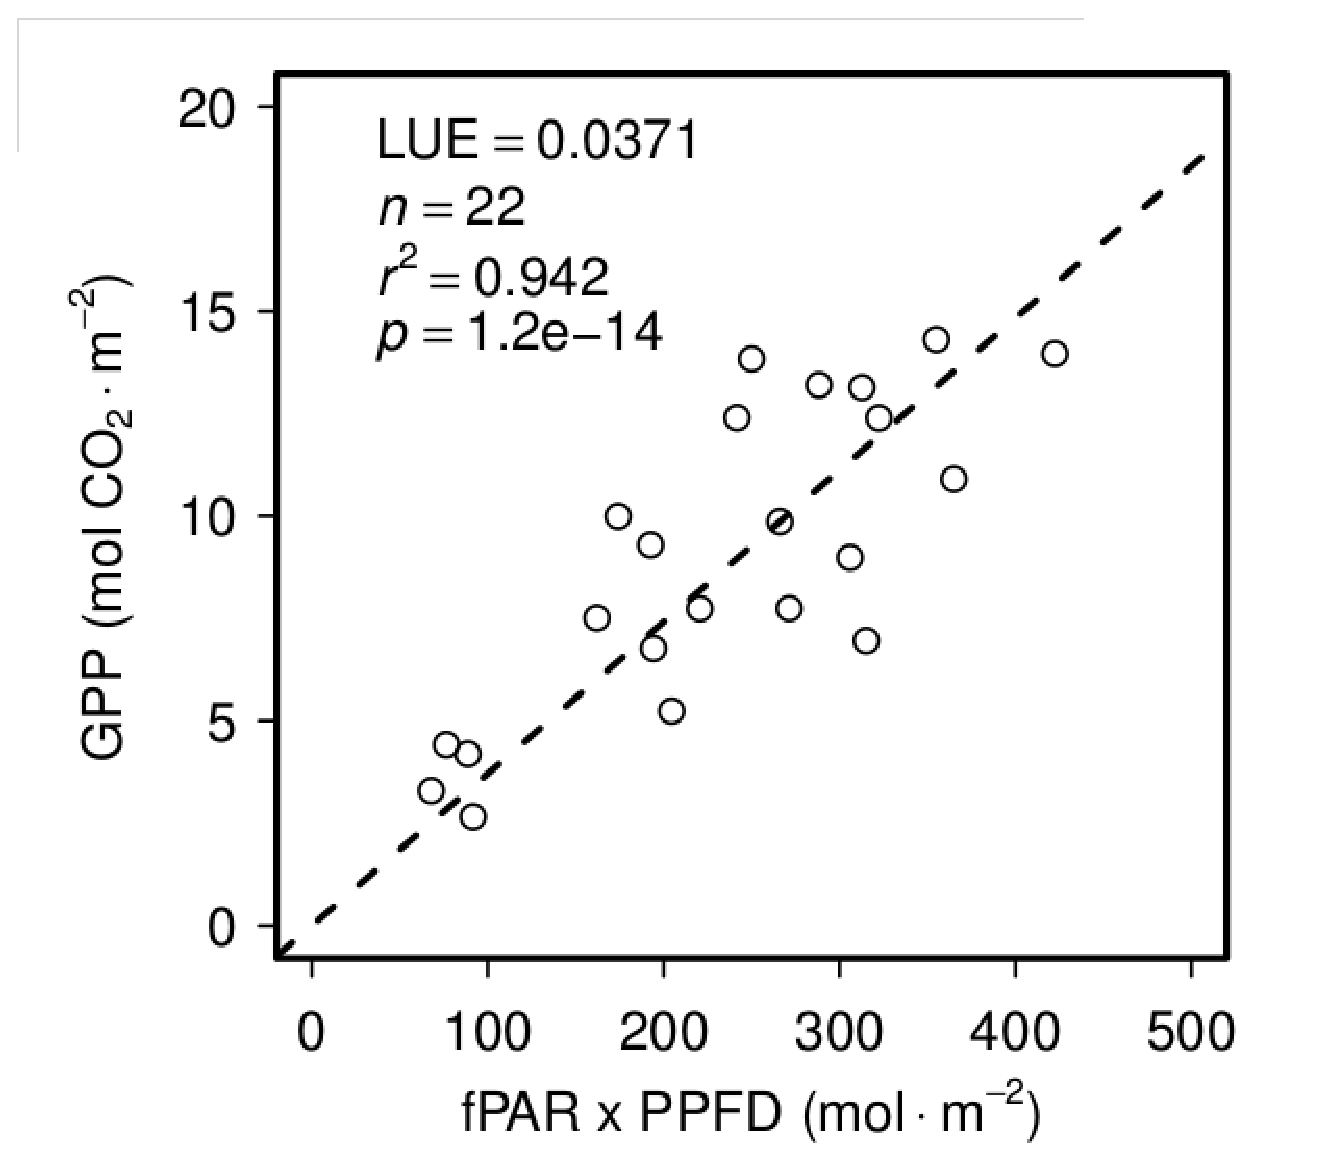
\includegraphics[width=0.55\textwidth]{lue_caqfo.eps}
    \caption{Light-use efficiency estimation based on the linear regression 
    between monthly aggregated GPP and fPAR $\times$ PPFD for station CA-Qfo, 
    Canada.}
    \label{fig:lue}
\end{figure}

%% \\\\\\\\\\\\\\\\\\\\\\\\\\\\\\\\\\\\\\\\\\\\\\\\\\\\\\\\\\\\\\\\\\\\\\\\ %%
%% PART 3.3.1 -- NEXT-GENERATION FORMULATION
%% //////////////////////////////////////////////////////////////////////// %%
\subsection{The ``next-generation'' formulation}
\label{sec:mst2nxtgen}

Following the successful implementation of the basic LUE model (in the GePiSaT model v1.0), it was discovered that information is still missing from the model described in Eq. \ref{eq:pem}. 
To address this problem, a ``next-generation'' model is proposed. 
This model, which is also a LUE model, can be expressed as follows \parencite[Eq. 8]{wang12}:
%% ------------------------------------------------------------------------ %%
%% eq:nglue | Production efficiency model
%% ------------------------------------------------------------------------ %%
\nomenclature{$\phi_{\circ}$}{Intrinsic quantum efficiency [mol CO$_{2}\cdot$m$^{-2}\cdot$mol PPFD$^{-1}$]}%
\nomenclature{$\alpha^{\star}$}{Cramer-Prentice bioclimatic moisture index}
\begin{equation}
\label{eq:nglue}
    \text{GPP} = \phi_{\circ} \cdot \alpha^{\star} \cdot \text{fPAR} \cdot
                 m \cdot \text{PPFD}
\end{equation}

\noindent where:\\
\indent $\phi_{\circ}$ = intrinsic quantum efficiency [mol CO$_{2}\cdot$m$^{-2}\cdot$mol PPFD$^{-1}$]\\
\indent $\alpha^{\star}$ = Cramer-Prentice bioclimatic moisture index\\
\indent $m$ = water-and-light-use compensation coefficient\\

It can be seen that Eq. \ref{eq:nglue} is a modified version of Eq. \ref{eq:pem}, where the basic LUE model has been fitted with additional parameters.  
In Eq. \ref{eq:nglue}, the basic LUE (i.e., $\varepsilon$) has been replaced with the intrinsic quantum efficiency, $\phi_{\circ}$. The effects of soil moisture on the LUE is incorporated with the addition of the Cramer-Prentice $\alpha^{\star}$ \parencite{prentice93, gallego-sala10}.  
For calculation details on $\alpha^{\star}$, see \S \ref{sec:gepcp}.

The water-and-light use compensation term, $m$, is defined as:
%% ------------------------------------------------------------------------ %%
%% eq:m | The Chi Term in LUE
%% ------------------------------------------------------------------------ %%
\nomenclature{$\chi$}{$c_{i}/c_{a}$ ratio}%
\nomenclature{$\gamma$}{$\Gamma^{\star}/c_{a}$ ratio}
\begin{equation}
\label{eq:m}
    m = \left( \frac{\chi - \gamma}{\chi + 2 \gamma}  \right) 
\end{equation}

\noindent where: \\
\indent $\chi$ = $c_{i}/c_{a}$ ratio\\
\indent $\gamma$ = $\Gamma^{\star}/c_{a}$ ratio \\

\noindent The new theoretically-based LUE model also introduces two new unitless parameters, $\chi$ and $\gamma$. 
The first parameter, $\chi$ represents the $c_{i}/c_{a}$ ratio (i.e., the ratio of intercellular leaf CO$_2$ concentration to the CO$_2$ concentration outside the leaf). 
A theory for predicting the leaf stomatal conductance can be used to express this ratio \parencite[Eq. 8]{prentice14}:
%% ------------------------------------------------------------------------ %%
%% eq:chi | ci/ca ratio
%% ------------------------------------------------------------------------ %%
\nomenclature{$\Gamma^{\star}$}{Photorespiratory compensation point [Pa]}%
\nomenclature{$c_a$}{Ambient CO$_2$ concentration [Pa]}%
\nomenclature{$\xi$}{Carbon cost of water}%
\begin{equation}
\label{eq:chi}
    \chi = \frac{\Gamma^{\star}}{c_{a}} + \left(1 - \frac{\Gamma^{\star}}{c_{a}} \right) \cdot \frac{\xi}{\xi + \sqrt{\text{VPD}}} 
\end{equation}

\noindent where:\\
\indent $\Gamma^{\star}$ = photorespiratory compensation point [Pa]\\
\indent $c_{a}$ = ambient CO$_2$ concentration [Pa]\\
\indent VPD = vapor pressure deficit [Pa]\\
\indent $\xi$ = carbon cost of water\\


%
% @TODO: incorporate conversion of CO2 to ca (ppm to Pa) somehow
%
The concentration data can be converted to partial pressure, knowing the total atmospheric pressure, using Dalton's Law of Partial Pressure:
%% ---------------------------------------------------------------%%
%% eq:pp | Partial Pressure Convertion
%% ---------------------------------------------------------------%%
\begin{equation}
\label{eq:pp}
    p_x = ppm_x \times 10^{-6} \times P_{atm}\left( z \right)
\end{equation}

\noindent where:\\
\indent $p_x$ = partial pressure of gas \textit{x} [Pa]\\
\indent $ppm_x$ = parts-per-million concentration of gas \textit{x} [ppm]\\
\indent $P_{atm}\left( z \right)$ = atmospheric pressure at elevation \textit{z} [Pa]\\



\noindent The carbon cost of water is expressed as \parencite{prentice14}:
%% ------------------------------------------------------------------------ %%
%% eq:xi | Carbon cost of water
%% ------------------------------------------------------------------------ %%
\nomenclature{$b/a$}{Ratio of unit cost of carboxylation to transpiration}%
\nomenclature{$K$}{Michaelis-Menten photosynthesis coefficient [Pa]}
\begin{equation}
\label{eq:xi}
    \xi = \sqrt{\frac{b}{a} \cdot \frac{K + \Gamma^{\star}}{1.6}}
\end{equation}

\noindent where: \\
\indent $b/a$ = ratio of the unit cost of carboxylation to transpiration\\
\indent $K$ = Michaelis-Menten coefficient in Rubisco-limited photosynthesis [Pa]\\

\noindent By substituting $\chi$ in Eq. \ref{eq:chi} and $\xi$ in Eq. \ref{eq:xi}, the $m$ term in Eq. \ref{eq:nglue} can be expressed as a function of $b/a$.  
The derivation has been left out; however, the simplified expression for $m$ is given by:
%% ------------------------------------------------------------------------ %%
%% eq:msimp | The simplification of m
%% ------------------------------------------------------------------------ %%
\begin{equation}
\label{eq:msimp}
    m = \frac{c_a - \Gamma^{\star}}{c_a + 2 \Gamma^{\star} 
    + 3 k \Gamma^{\star} \cdot \sqrt{D} \cdot 
    \left( b/a \right)^{-0.5} \cdot \left( K + \Gamma^{\star} \right)^{-0.5}}
\end{equation}

\noindent where: \\
\indent $k = \sqrt{1.6} \approx 1.26$ \\

The Michaelis-Menten coefficient of Rubisco-limited photosynthetic rate is a function of the Rubisco photosynthetic rates for O$_2$ and CO$_2$ \parencite{farquhar80}:
%% ------------------------------------------------------------------------ %%
%% eq:michaelis | Michaelis Menten coefficient
%% ------------------------------------------------------------------------ %%
\nomenclature{$K_c$}{Michaelis-Menten constant for carboxylation [Pa]}%
\nomenclature{$K_o$}{Michaelis-Menten constant for oxygenation [Pa]}%
\nomenclature{$O_i$}{Partial pressure of O$_2$ concentration [Pa]}
\begin{equation}
\label{eq:michaelis}
	K=K_c \cdot \left( 1 + \frac{O_i}{K_o} \right)
\end{equation}

\noindent where:\\
\indent $K_c$ = Michaelis-Menten constant for carboxylation [Pa]\\
\indent $K_o$ = Michaelis-Menten constant for oxygenation [Pa]\\
\indent $O_i$ = oxygen concentration [Pa]\\

\noindent The photorespiratory compensation point (i.e., $\Gamma^{\star}$ in Eq. \ref{eq:chi}) and both Michaelis-Menten constants (i.e., $K_c$ and $K_o$ in Eq. \ref{eq:michaelis}) have temperature dependencies \parencite{farquhar80}.  
The temperature dependencies of these constants have been fit to the Arrhenius function and were normalized with respect to 25$^{\circ}$C:
%% ------------------------------------------------------------------------ %%
%% eq:kckogs | Michaelis Menten Kc & Ko coefficients
%% ------------------------------------------------------------------------ %%
\nomenclature{$K_{c25}$}{Michaelis-Menten constant for carboxylation at 25$^{\circ}$C}%
\nomenclature{$K_{o25}$}{Michaelis-Menten constant for oxygenation at 25$^{\circ}$C}%
\nomenclature{$\Gamma^{\star}_{25}$}{Photorespiratory compensation point at 25$^{\circ}$C}%
\nomenclature{$\Delta H_c$}{Energy of activation for carboxylation [kJ$\cdot$mol$^{-1}$]}%
\nomenclature{$\Delta H_o$}{Energy of activation for oxygenation [kJ$\cdot$mol$^{-1}$]}%
\nomenclature{$\Delta H_{\Gamma^{\star}}$}{Energy of activation for $\Gamma^{\star}$ [kJ$\cdot$mol$^{-1}$]}%
\nomenclature{$T_k$}{Leaf temperature [K]}
\begin{subequations}
\label{eq:kckogs}
\begin{align}
        K_o&=K_{o25} \cdot \exp \left( 
             \frac{\Delta H_o \cdot \left( T_k-298 \right)}
                  {298 \cdot R_{u} \cdot T_k}
             \right) \label{eq:ko} \\
        K_c&=K_{c25} \cdot \exp \left( 
             \frac{\Delta H_c \cdot \left( T_k-298 \right)}
                  {298 \cdot R_{u} \cdot T_k}
             \right) \label{eq:kc} \\
        \Gamma^{\star}&=\Gamma^{\star}_{25} \cdot \exp \left(
			\frac{\Delta H_{\Gamma^{\star}} \cdot \left( T_k - 298 \right)}
			     {298 \cdot R_{u} \cdot T_k} 	
        	\right) \label{eq:gs}
\end{align}
\end{subequations}

\noindent where:\\
\indent $K_{c25}$ = Michaelis-Menten constant for carboxylation at 25$^{\circ}$C\\
\indent $K_{o25}$ = Michaelis-Menten constant for oxygenation at 25$^{\circ}$C\\
\indent $\Gamma^{\star}_{25}$ = Photorespiratory compensation point at 25$^{\circ}$C\\
\indent $\Delta H_c$ = energy of activation for carboxylation [kJ$\cdot$mol$^{-1}$]\\
\indent $\Delta H_o$ = energy of activation for oxygenation [kJ$\cdot$mol$^{-1}$]\\
\indent $\Delta H_{\Gamma^{\star}}$ = energy of activation for $\Gamma^{\star}$\\
\indent $T_k$ = leaf temperature [K]\\
\indent $R_{u}$ = universal gas constant, 8.314 [J$\cdot$mol$^{-1}\cdot$K$^{-1}$]\\

\noindent The Michaelis-Menten constants, $K_{o25}$ and $K_{c25}$, and their associated activation energies (i.e., $\Delta H_o$ and $\Delta H_c$, respectively) as well as the photorespiratory compensation point, $\Gamma^{\star}$, and its activation energy have been determined by experimentally fitted data \parencite{farquhar80, bernacchi01}.  
Table \ref{tab:michaelis} lists published values for the constants used in Eqs. \ref{eq:ko}--\ref{eq:gs}.
%% ------------------------------------------------------------------------ %%
%% tab:michaelis | Kc25 & Ko25 constants
%% ------------------------------------------------------------------------ %%
\begin{table}[h]
    \caption{Temperature response curve constants.}
    \label{tab:michaelis}
    \centering
    \begin{tabular}{l l l}
        \toprule
        \bf{Constant} & \bf{Value} & \bf{Reference} \\
        \toprule
        $K_{c25}$ [Pa] & 46 & Farquhar et al., 1980 \\
        
        ~ & 41\textsuperscript{*} & Bernacchi et al., 2001 \\
        
        $K_{o25}$ [kPa] & 33.0 & Farquhar et al., 1980 \\
        
        ~ & 28.2\textsuperscript{*} & Bernacchi et al., 2001 \\
        
        $\Gamma^{\star}_{25}$ [Pa] & 3.1 & Farquhar et al., 1980 \\
        
        ~ & 4.3\textsuperscript{*} & Bernacchi et al., 2001 \\
        
        $\Delta H_c$ [kJ$\cdot$mol$^{-1}$] & 59.356 & Farquhar et al., 1980 \\
        
        ~ & 79.43 & Bernacchi et al., 2001 \\
        
        $\Delta H_o$ [kJ$\cdot$mol$^{-1}$] & 35.948 & Farquhar et al., 1980 \\
        
        ~ & 36.38 & Bernacchi et al., 2001 \\
        
        $\Delta H_{\Gamma^{\star}}$ [kJ$\cdot$mol$^{-1}$] & 37.83 & Bernacchi et al., 2001\\
        
        \multicolumn{3}{l}{
        	\footnotesize{*assumes experiments performed at 
        	25$^{\circ}$C and 101.3 kPa}
        	}\\
        \bottomrule
    \end{tabular}
\end{table}

%% ------------------------------------------------------------------------ %%
%% fig:michaelis | Bernacchi v Farquhar Michaelis-Menten constants
%% ------------------------------------------------------------------------ %%
\begin{figure}[h!]
	\centering
    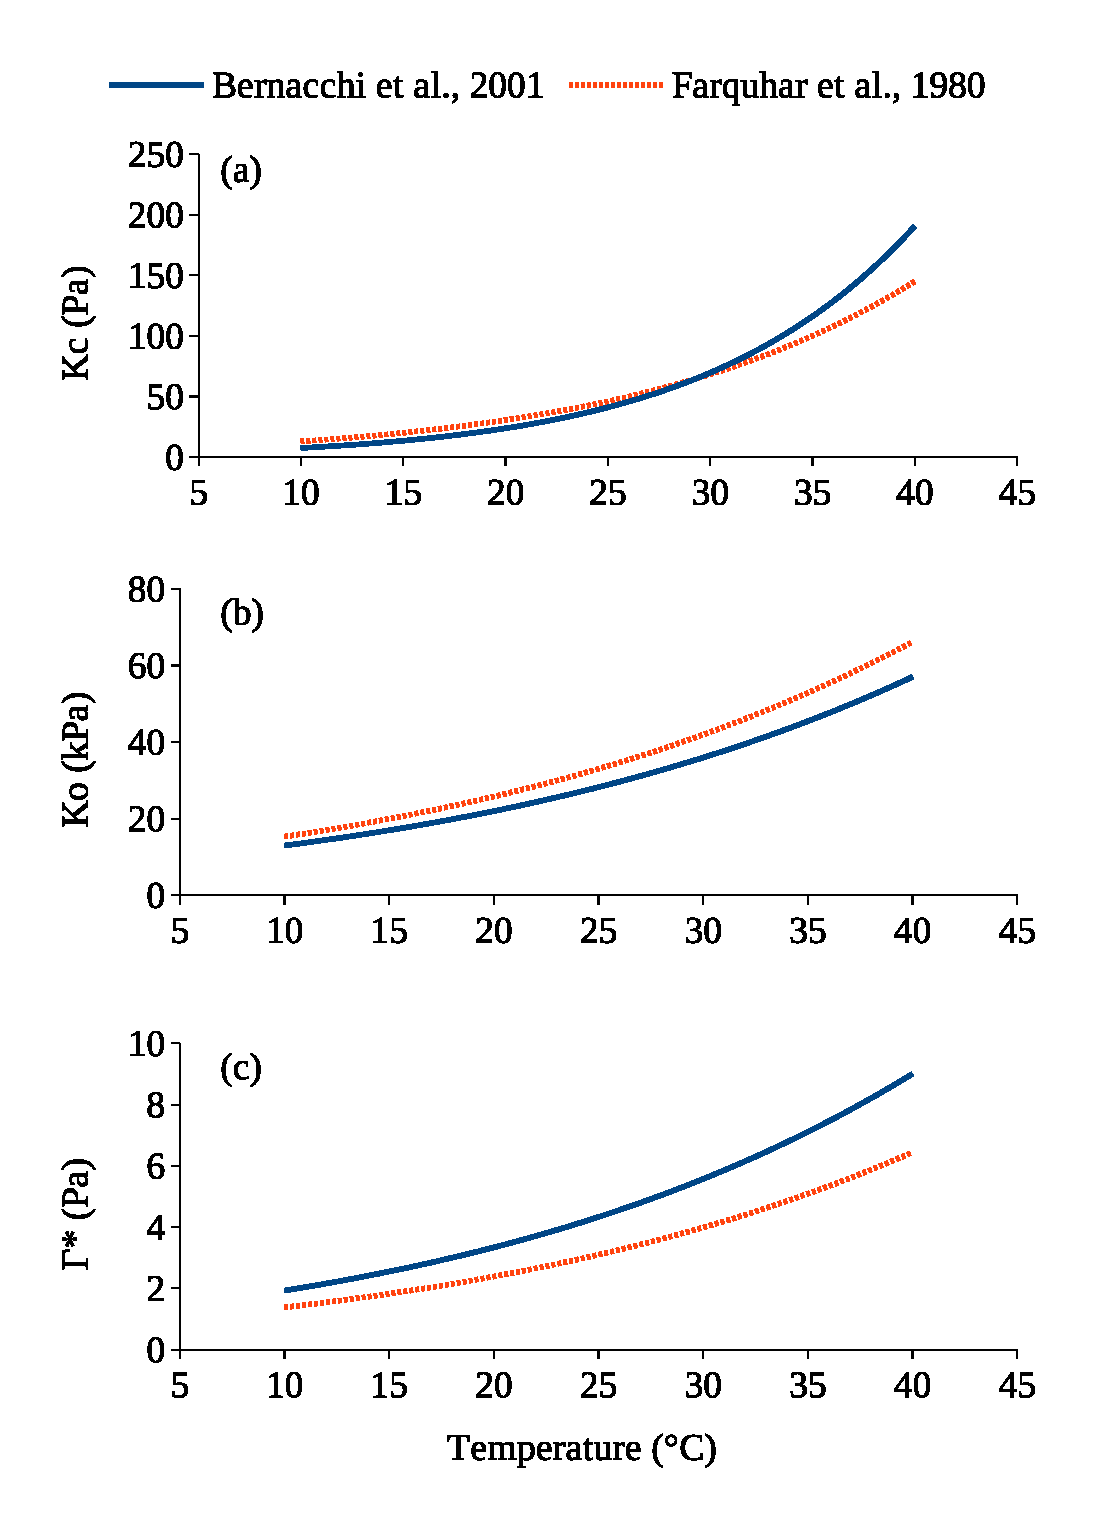
\includegraphics[width=0.8\textwidth]{michaelis.eps}
    \caption{Plots of the temperature response curves of the Michaeli-Menten 
    constants (a) $K_c$ and (b) $K_o$ and (c) the photorespiratory compensation 
    point, $\Gamma^{\star}$ using the constants from Table \ref{tab:michaelis}
    reported by Bernacchi et al., 2001 (solid blue) and Farquhar et al., 1980 
    (dashed red).}
    \label{fig:michaelis}
\end{figure}

\noindent Figure \ref{fig:michaelis} shows the comparison between the temperature response curves of the values given in Table \ref{tab:michaelis}.  
A stronger response in $K_c$ can be seen for the Bernacchi et al., 2001 response curve (Fig. \ref{fig:michaelis}a, solid blue) compared to the Farquhar et al., 1980 curve (dashed red).  
The more curvilinear appearance is due to a higher energy of activation, $\Delta H_c$ (79.43 compared to 59.356 kJ$\cdot$mol$^{-1}$). 
The temperature response curve for Farquhar et al., 1980 reports higher values of $K_o$ compared to Bernacchi et al., 2001 across all temperatures.  
The opposite relationship is true for $\Gamma^{\star}$ where the Bernacchi et al., 2001 response curve is greater than the Farquhar et al., 1980 response curve.  
In all three  temperature response curves, the deviation between the Bernacchi et al., 2001 and Farquhar et al., 1980 increases with temperature; especially visible at high temperatures (i.e., $>30^{\circ}$C). 
For the purposes of this model, the values reported by Bernacchi et al., 2001 in Table \ref{tab:michaelis} are used.  

%
% @TODO: incorporate barometric formula somehow 
%
Atmospheric pressure as a function of elevation can be calculated with the following \parencite{cavcar00}:
%% ---------------------------------------------------------------%%
%% eq:pz | Atmospheric pressure as a function of elevation
%% ---------------------------------------------------------------%%
\nomenclature{$P_{\circ}$}{Base atmospheric pressure, 101325 [Pa]}%
\nomenclature{$L$}{Temperature lapse rate, 0.0065 [K$\cdot$m$^{-2}$]}%
\nomenclature{$z$}{Altitude [m]}%
\nomenclature{$T_{\circ}$}{Base temperature, 298.15 [K]}%
\nomenclature{$g$}{Acceleration of gravity, 9.81 [m$\cdot$s$^{-2}$]}%
\nomenclature{$M_a$}{Molecular weight of dry air, 0.028963 [kg$\cdot$mol$^{-1}$]}%
\nomenclature{$R_u$}{Universal gas constant, 8.314 [J$\cdot$mol$^{-1}\cdot$K$^{-1}$]}
\begin{equation}
\label{eq:pz}
    P_{atm}\left( z \right) = P_{\circ} \cdot \left( 
    	1 - \frac{L \cdot z}{T_{\circ}} 
    \right)^{\frac{g \cdot M_a}{R_u \cdot L}}
\end{equation}

\noindent where:\\
\indent $P_{\circ}$ = base atmospheric pressure [101325 Pa]\\
\indent $L$ = temperature lapse rate [0.0065 K$\cdot$m$^{-2}$]\\
\indent $z$ = altitude [m]\\
\indent $T_{\circ}$ = base temperature [298.15 K]\\
\indent $g$ = acceleration due to gravity [9.81 m$\cdot$s$^{-2}$]\\
\indent $M_a$ = molecular weight for dry air [0.028963 kg$\cdot$mol$^{-1}$]\\
\indent $R_u$ = universal gas constant [8.314 J$\cdot$mol$^{-1}\cdot$K$^{-1}$]\\


%% \\\\\\\\\\\\\\\\\\\\\\\\\\\\\\\\\\\\\\\\\\\\\\\\\\\\\\\\\\\\\\\\\\\\\\\\ %%
%% PART 3.3.2 -- GAP-FILLED PPFD
%% //////////////////////////////////////////////////////////////////////// %%
\subsection{Gap-filling the PPFD observations}
\label{sec:mst2gfppfd}
One of the principle objectives of this project is to use observation data when and where it is available.  
However, there are times when observation data is limited or simply unavailable; therefore, a substitute is required. 

In order to compute the monthly GPP aggregates, the complete time series of GPP is necessary.  
Due to gaps present in the flux tower datasets, a gap-filling product is used to complete the PPFD time series.
%% ------------------------------------------------------------------------ %%
%% fig:gapfill | PPFD gap-filling example
%% ------------------------------------------------------------------------ %%
\begin{figure}[h!]
    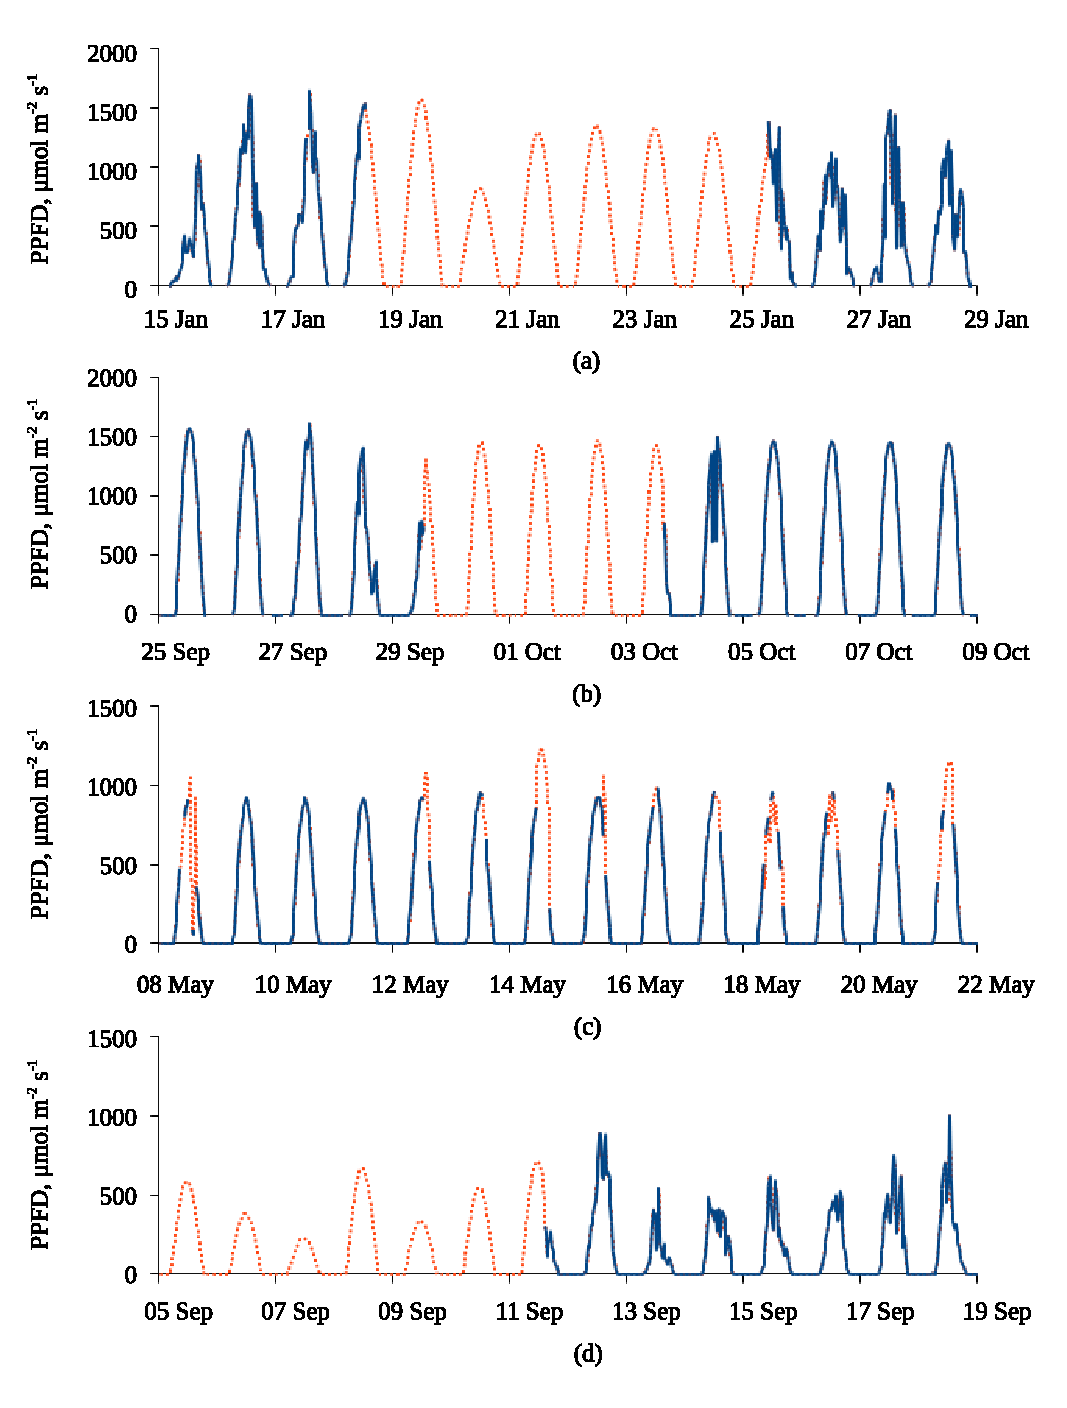
\includegraphics[width=0.95\textwidth]{gapfill.eps}
    \caption{Plots of two-week periods during 2002 of half-hourly PPFD 
    observations (solid blue) and gap-filling product (dashed red) for flux 
    tower stations: (a) DK-Sor, Denmark; (b) US-Blo, United States; (c) BR-Sa3, 
    Brazil; (d) RU-Zot, Russia.}
    \label{fig:gapfill}
\end{figure}

Flux tower measurements are made at a half-hourly time step; therefore the gap-filling product will be computed at this same time resolution.  
The gap-filling product begins with the calculation of half-hourly extraterrestrial solar radiation (see \S \ref{sec:mst2efpar}).  
For each day where PPFD is being gap-filled, the 24-hour extraterrestrial solar radiation time series (at half-hourly time step) is computed based on Eq. \ref{eq:etsr}. 
The daily integrated total extraterrestrial solar radiation is also computed.  
To scale the magnitude of the extraterrestrial solar radiation for the land surface, the daily $SW_{down}$ observation for the same day and location of the flux tower is used.  
To convert the time series from units of energy to units of flux, a from-flux-to-energy conversion efficiency coefficient (fFEC) is used \parencite{ge11}. 
The scaled and converted daily time series of extraterrestrial solar radiation serves as the gap-filling product and is described in the following equation:
%% ------------------------------------------------------------------------ %%
%% eq:gapfill | PPFD gapfilling product
%% ------------------------------------------------------------------------ %%
\nomenclature{$Q_{gap}$}{PPFD gap-filling product [$\mu$mol$\cdot$m$^{-2}\cdot$s$^{-1}$]}%
\nomenclature{$\text{fFEC}$}{From-flux-to-energy conversion efficiency [$\mu$mol$\cdot$J$^{-1}$]}
\begin{equation}
\label{eq:gapfill}
    Q_{gap} = \text{fFEC} \cdot 
              \frac{\int_{day} SW_{down}}{\int_{day} R_a} \cdot R_a
\end{equation}

\noindent where:\\
\indent $Q_{gap}$ = half-hourly PPFD gap-filling product [$\mu$mol$\cdot$m$^{-2}\cdot$s$^{-1}$]\\ 
\indent fFEC = from-flux-to-energy conversion efficiency [$\mu$mol$\cdot$J$^{-1}$]\\
\indent $R_a$ = half-hourly extraterrestrial solar radiation [W$\cdot$m$^{-2}$]\\

\noindent After the creation of the daily gap-filling product, the original observation data is overlain the time series thus creating the half-hourly gap-filled observation time series.  
There are several different values for the fFEC coefficient including 2.27 $\mu$mol$\cdot$J$^{-1}$ \parencite{prentice93}, 2.16 $\mu$mol$\cdot$J$^{-1}$ \parencite{ge11}, and 2.04 $\mu$mol$\cdot$J$^{-1}$ \parencite{meek84}. 
For a conservative approach, the value of 2.04 $\mu$mol$\cdot$J$^{-1}$ is used in Eq. \ref{eq:gapfill}.

Figure \ref{fig:gapfill} shows and example of the gap-filling procedure applied to four flux towers of two-week periods during 2002.  
PPFD observations (deplicted as a solid blue line) are gap-filled (shown as dashed red lines) during periods where observations are missing.  
The results shown in Figure \ref{fig:gapfill} suggest that the gap-filling procedure presented above adequately reproduces diurnal cycling with magnitudes and durations representative of the surrounding observations.  
Furthermore, the daily $SW_{down}$ measurements seem to capture the inter-daily variability of the PPFD observations (Figures \ref{fig:gapfill} a and d). 
However, the gap-filling product does not account for sub-daily variability due to the smooth curve represented by the extraterrestrial solar radiation.

%% \\\\\\\\\\\\\\\\\\\\\\\\\\\\\\\\\\\\\\\\\\\\\\\\\\\\\\\\\\\\\\\\\\\\\\\\ %%
%% PART 3.3.1.1 -- ET SOLAR RADIATION
%% //////////////////////////////////////////////////////////////////////// %%
\subsubsection{Calculating extraterrestrial solar radiation}
\label{sec:mst2etsr}
To gap-fill the half-hourly PPFD time curve, it is first assumed that the diurnal PPFD curve follows the general trend of solar energy over the course of the day. 
There are several models describing the sub-daily solar energy curve \parencite{ahmad11}.  
For the purposes of this project, the idealized extraterrestrial solar radiation curve will be used.  
Daily effects of clouds and other atmospheric particulates will be taken into account during the scaling with WATCH $SW_{down}$.  
Sub-daily variability is not accounted for utilizing this method; however, due to the fact that these data will be processed into monthly aggregates, sub-daily variability was not considered important in this model. 

The equation for calculating the extraterrestrial solar radiation is as follows \parencite[Eq.~1.10.2]{duffie13}:
%% ------------------------------------------------------------------------ %%
%% eq:etsr | Extraterrestrial Solar Radiation
%% ------------------------------------------------------------------------ %%
\nomenclature{$R_{a}$}{Extraterrestrial solar radiation [W$\cdot$m$^{-2}$]}%
\nomenclature{$G_{sc}$}{Solar constant, 1367 W$\cdot$m$^{-2}$}%
\nomenclature{$d_{r}$}{Earth's orbit eccentricity correction factor}%
\nomenclature{$\phi$}{Observer's latitude [radians]}%
\nomenclature{$\delta$}{Earth's declination angle [radians]}%
\nomenclature{$\omega$}{Solar angle [radians]} 
\begin{equation}
\label{eq:etsr}
    R_{a} = G_{sc} \cdot d_{r} \cdot \left(\cos \phi \cdot \cos \delta \cdot \cos \omega + \sin \phi \cdot \sin \delta\right)
\end{equation}

\noindent where: \\
\indent $R_{a}$ = extraterrestrial solar radiation \\
\indent $G_{sc}$ = solar constant \\
\indent $d_{r}$ = Earth's orbit eccentricity correction factor \\
\indent $\phi$ = latitude of observation [radians]\\
\indent $\delta$ = Earth's declination angle [radians] \\
\indent $\omega$ = solar angle [radians] \\

\noindent The solar constant, $G_{sc}$, that is adopted for use in this study is 1367~W$\cdot$m$^{-2}$ (i.e., 1.960~cal$\cdot$cm$^{-2}\cdot$min$^{-1}$, 433~btu$\cdot$ft$^{-2}\cdot$h$^{-1}$, 4.921~MJ$\cdot$m$^{-2}\cdot$h$^{-1}$) \parencite{duffie13,wehrli85}.  
The correction factor for the eccentricity of Earth's orbit around the sun is given by \parencite{spencer71}:
%% ------------------------------------------------------------------------ %%
%% eq:dr | Earth's orbit eccentricity correction
%% ------------------------------------------------------------------------ %%
\nomenclature{$J_{doy}$}{Julian day of the year}%
\nomenclature{$D$}{Total number of days in a year}
\begin{equation}
\label{eq:dr}
    d_{r} = 1.0 + 0.033 \cdot \cos \left(\frac{2\pi J_{doy}}{D}\right)
\end{equation}

\noindent where: \\
\indent $J_{doy}$ = Julian day of the year (1--366) \\
\indent $D$ = total number of days in the year (365.242) \\

\noindent Earth's declination angle (ranging from -23.45 during the winter solstice to 23.45 during the summer solstice) is given by \parencite{cooper69}:

%% ------------------------------------------------------------------------ %%
%% eq:delta | Earth's declination angle
%% ------------------------------------------------------------------------ %%
\begin{equation}
\label{eq:delta}
    \delta = 23.45 \cdot \sin \left(\frac{2\pi}{D}\cdot (284 + J_{doy})\right)
\end{equation}

\noindent The solar angle, in degrees, ranges from -180$^{\circ}$ to 180$^{\circ}$ with 0$^{\circ}$ occurring at solar noon and is given by \parencite[Eq. 3.1]{stine01}:
%% ------------------------------------------------------------------------ %%
%% eq:omega | Solar angle
%% ------------------------------------------------------------------------ %%
\nomenclature{$t_{s}$}{Solar time [h]}
\begin{equation}
\label{eq:omega}
    \omega = 15 \cdot (t_{s} - 12)
\end{equation}

\noindent where: \\
\indent $t_{s}$ = solar time [h] \\

\noindent The conversion between local clock time ($LCT$) and solar time ($t_{s}$) depends on the physical observation location, the day of the year, and the time zone of the location.  
The conversion equation takes the form \parencite[Eq. 3.5]{stine01}:
%% ------------------------------------------------------------------------ %%
%% eq:soltime | Solar time
%% ------------------------------------------------------------------------ %%
\nomenclature{$LCT$}{Local clock time [h]}%
\nomenclature{$EOT$}{Equation of time [min]}%
\nomenclature{$LC$}{Longitude correction factor [h]}
\begin{equation}
\label{eq:soltime}
    t_{s} = LCT + \frac{EOT}{60} - LC
\end{equation}

\noindent where: \\
\indent $LCT$ = local clock time [h] \\
\indent $EOT$ = equation of time [min] \\
\indent $LC$ = longitude correction factor [h] \\

\noindent The equation of time ($EOT$) is the measure of difference between the mean solar time and the true solar time.  
Due to the seasonal changes which account for the mean solar time, the actual solar time can be as great at $\pm$17 min from the mean \parencite{stine01}.  
An approximation of $EOT$ is given by \parencite{stine01,woolf68}:
%% ------------------------------------------------------------------------ %%
%% eq:eot | Equation of time
%% ------------------------------------------------------------------------ %%
\nomenclature{$B$}{In equation of time, $B$ = $2\pi \cdot (J_{doy}-1) \cdot D^{-1}$}
\begin{equation}
\label{eq:eot}
    EOT = 0.258 \cdot \cos B - 7.416 \cdot \sin B - 3.648 \cdot \cos (2B) - 9.228 \cdot \sin (2B)
\end{equation}

\noindent where: \\
\indent $B$ = $2\pi \cdot (J_{doy}-1) \cdot D^{-1}$ \\

\noindent The longitude correction factor ($LC$) makes the appropriate adjustment for the local time zone difference from the UTM/GMT based on the rotational speed of the Earth (15$^{\circ}$ longitude$\cdot$h$^{-1}$) and is given by \parencite{stine01}:
%% ------------------------------------------------------------------------ %%
%% eq:lc | Longitude correction factor
%% ------------------------------------------------------------------------ %%
\nomenclature{$TZ_{h}$}{Time-zone hours away from UTC [h]}%
\nomenclature{$lon$}{Observer's longitude [degrees]}
\begin{equation}
\label{eq:lc}
    LC = \frac{15 \cdot TZ_{h} - lon}{15}
\end{equation}

\noindent where: \\
\indent $TZ_{h}$ = number of time zones away from UTC [h] \\
\indent $lon$ = longitude of observation [degrees] \\

Equation \ref{eq:etsr} can now be solved for any set of values consisting of a longitude ($lon$), latitude ($\phi$), and day of the year ($J_{doy}$).  
If $LC$ in equation \ref{eq:soltime} is the half-hourly time series for a given day (i.e., 0.0--23.5 h), $R_{a}$ will be the half-hourly extraterrestrial solar radiation in W$\cdot$m$^{-2}$.  
For consistency with the PPFD values which these values will be gap-filling, units of solar radiation must be converted to units of photon flux density.  
The conversion factor from W$\cdot$m$^{-2}$ to $\mathrm{\mu}$mol$\cdot$m$^{-2}\cdot$s$^{-1}$ is 2.04~$\mathrm{\mu}$mol$\cdot$J$^{-1}$ \parencite{meek84,chen93}.

%% \\\\\\\\\\\\\\\\\\\\\\\\\\\\\\\\\\\\\\\\\\\\\\\\\\\\\\\\\\\\\\\\\\\\\\\\ %%
%% PART 3.3.3 -- ESTIMATING fPAR
%
% @ TODO: change section to estimating Iabs
%
%% //////////////////////////////////////////////////////////////////////// %%
\subsection{Estimating fPAR}
\label{sec:mst2efpar}
During photosynthesis, pigments within plant leaves (e.g., chlorophyll and carotenoids) absorb $SW_{down}$ (0.30--3.00~$\mathrm{\mu}$m) particularly well the wavelengths within the blue and red visible spectrum (0.40--0.51~$\mathrm{\mu}$m and 0.61--0.70~$\mathrm{\mu}$m, respectively).  
Light energy within this range (i.e., 0.40--0.70~$\mathrm{\mu}$m) has come to be known as photosynthecally active radiation (PAR) \parencite{oke87}.  
The fraction of available energy within the PAR-specific region of the electromagnetic spectrum ($\eta$) is approximately 50\% of the total $SW_{down}$ energy \parencite{stanhill77}.  
Therefore, PAR can be estimated based on $SW_{down}$ measurements:
%% ------------------------------------------------------------------------ %%
%% eq:sw2par | Shorwave radiation to PAR
%% ------------------------------------------------------------------------ %%
\nomenclature{$\text{PAR}$}{Photosynthetically active radiation (0.4--0.7 $\mu$m) [W$\cdot$m$^{-2}$]}%
\nomenclature{$\eta$}{Relative flux density of PAR [unitless]}%
\nomenclature{$SW_{down}$}{Shortwave downwelling radiation (0.3--3.0 $\mu$m) [W$\cdot$m$^{-2}$]}
\begin{equation}
\label{eq:sw2par}
    \text{PAR} = \eta \cdot SW_{down}
\end{equation}

\noindent where:\\
\indent $SW_{down}$ = shortwave downwelling radiation [W$\cdot$m$^{-2}$]\\
\indent PAR = photosynthetically active radiation [W$\cdot$m$^{-2}$]\\
\indent $\eta$ = relative flux density of PAR\\

\noindent Not all of the energy available within the PAR waveband is absorbed by the vegetation canopy.  
Therefore, it is often considered more important to investigate the fraction of absorbed PAR (fPAR).  
Process-based methods of estimating fPAR often rely on some type of vegetation index (e.g., leaf area or satellite-derived index).  
